\documentclass[a4paper,12pt]{article} 

% First, we usually want to set the margins of our document. For this we use the package geometry.
\usepackage[top = 2.5cm, bottom = 2.5cm, left = 2.5cm, right = 2.5cm]{geometry} 
\usepackage[T1]{fontenc}
\usepackage[utf8]{inputenc}

% The following two packages - multirow and booktabs - are needed to create nice looking tables.
\usepackage{multirow} % Multirow is for tables with multiple rows within one cell.
\usepackage{booktabs} % For even nicer tables.

% As we usually want to include some plots (.pdf files) we need a package for that.
\usepackage{graphicx} 

% The default setting of LaTeX is to indent new paragraphs. This is useful for articles. But not really nice for homework problem sets. The following command sets the indent to 0.
\usepackage{setspace}
\setlength{\parindent}{0in}

% Package to place figures where you want them.
\usepackage{float}

% The fancyhdr package let's us create nice headers.
\usepackage{fancyhdr}

\usepackage{amsmath,amsthm,caption,amsfonts}
\usepackage[open]{bookmark}
\usepackage{minted}

\newcommand{\pard}[2]{\frac{\partial #1}{\partial #2}}


% To make our document nice we want a header and number the pages in the footer.

\pagestyle{fancy} % With this command we can customize the header style.

\fancyhf{} % This makes sure we do not have other information in our header or footer.

\lhead{\footnotesize Computer Network: Assignment 1}% \lhead puts text in the top left corner. \footnotesize sets our font to a smaller size.

%\rhead works just like \lhead (you can also use \chead)
\rhead{\footnotesize Mengxuan Wu} %<---- Fill in your lastnames.

% Similar commands work for the footer (\lfoot, \cfoot and \rfoot).
% We want to put our page number in the center.
\cfoot{\footnotesize \thepage} 

\begin{document}

\thispagestyle{empty} % This command disables the header on the first page. 

\begin{tabular}{p{15.5cm}}
{\large \bf Computer Network} \\
Southern University of Science and Technology \\ Mengxuan Wu \\ 12212006 \\
\hline
\\
\end{tabular}

\vspace*{0.3cm} %add some vertical space in between the line and our title.

\begin{center}
	{\Large \bf Assignment 1}
	\vspace{2mm}

	{\bf Mengxuan Wu}
		
\end{center}  

\vspace{0.4cm}

\section{Demonstration of the program}

In the following sections, figures of CLI are shown to demonstrate the program.
If two CLI are opened, the left one is the server and the right one is the client.
If only one CLI is opened, it is the client.

\subsection{Task 1}

\begin{figure}[H]
    \centering
    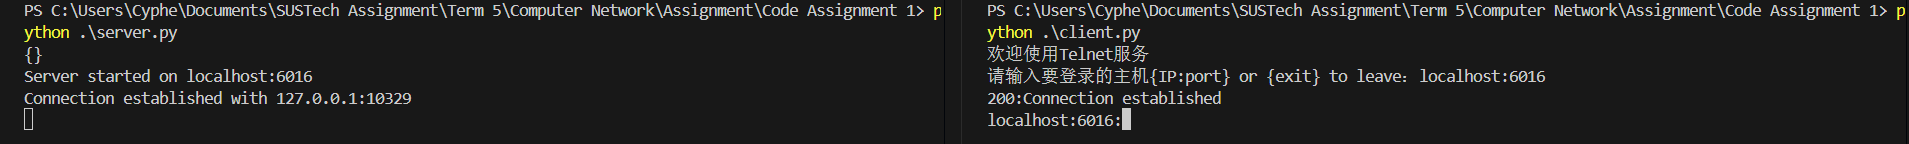
\includegraphics[width=\linewidth]{figure/task1.png}
    \caption{Initialization of the server and client}
\end{figure}

\subsection{Task 2}

\begin{figure}[H]
    \centering
    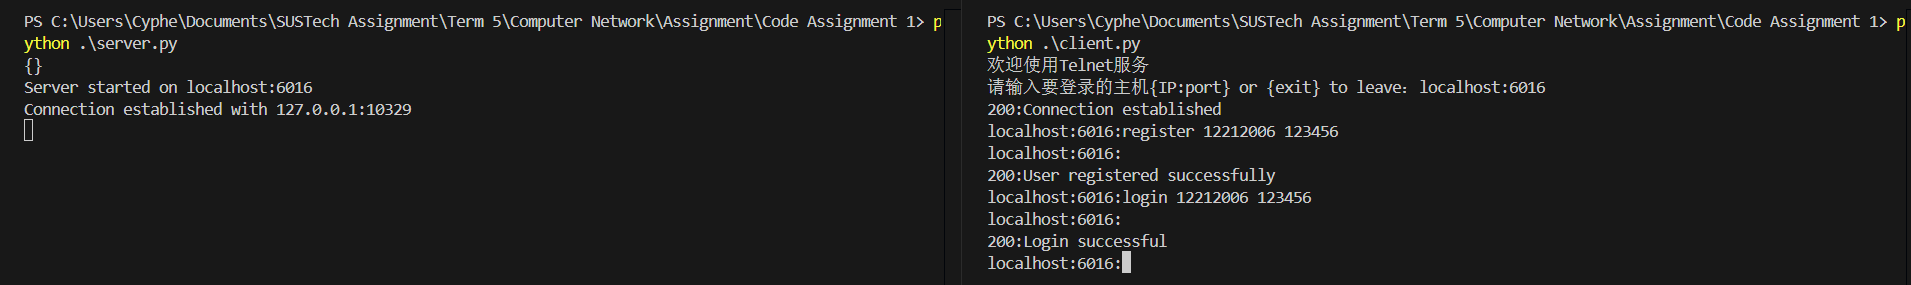
\includegraphics[width=\linewidth]{figure/task2.png}
    \caption{Register and login}
\end{figure}

\subsection{Task 3}

No image since all implementation is in the code.

\subsection{Task 4}

\begin{figure}[H]
    \centering
    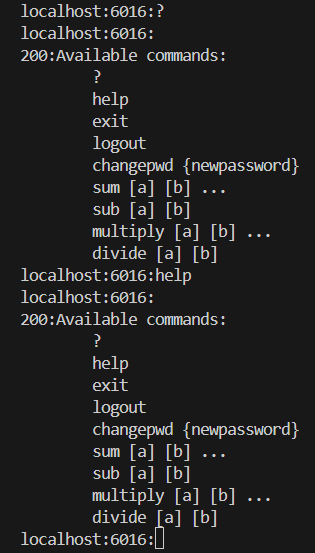
\includegraphics[width=0.3\linewidth]{figure/help.png}
    \caption{Help command}
\end{figure}

\begin{figure}[H]
    \centering
    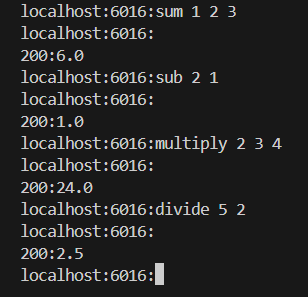
\includegraphics[width=0.3\linewidth]{figure/arithmetic.png}
    \caption{Arithmetic command}
\end{figure}

\begin{figure}[H]
    \centering
    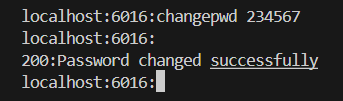
\includegraphics[width=0.3\linewidth]{figure/changepwd.png}
    \caption{Change password command}
\end{figure}

\begin{figure}[H]
    \centering
    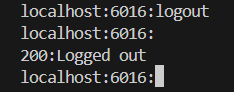
\includegraphics[width=0.3\linewidth]{figure/logout.png}
    \caption{Logout command}
\end{figure}

\begin{figure}[H]
    \centering
    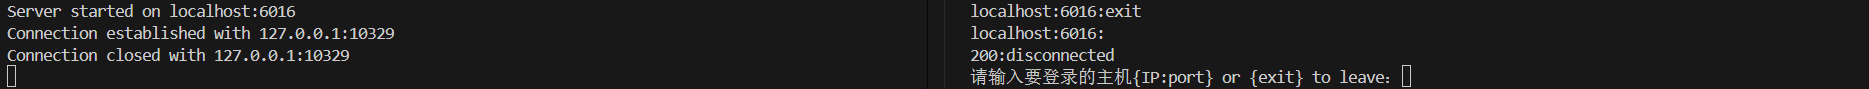
\includegraphics[width=\linewidth]{figure/exit.png}
    \caption{Exit command}
\end{figure}

\subsection{Task 5}

\begin{figure}[H]
    \centering
    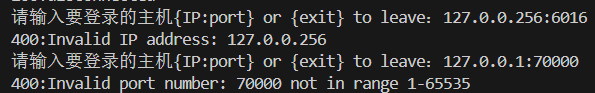
\includegraphics[width=0.5\linewidth]{figure/exception1.png}
    \caption{Invalid IP or port}
\end{figure}

\begin{figure}[H]
    \centering
    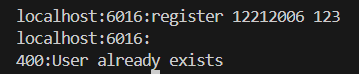
\includegraphics[width=0.5\linewidth]{figure/exception2.png}
    \caption{Attempt to register with an existing username}
\end{figure}

\begin{figure}[H]
    \centering
    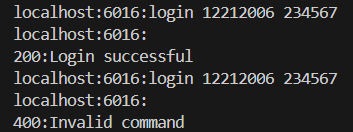
\includegraphics[width=0.5\linewidth]{figure/exception3.png}
    \caption{Attempt to login again after logging in}
\end{figure}

\begin{figure}[H]
    \centering
    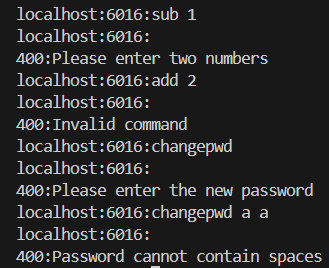
\includegraphics[width=0.5\linewidth]{figure/exception4.png}
    \caption{Too many or too few arguments}
\end{figure}

\begin{figure}[H]
    \centering
    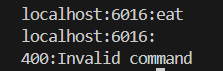
\includegraphics[width=0.5\linewidth]{figure/exception4.1.png}
    \caption{Command does not exist}
\end{figure}

\begin{figure}[H]
    \centering
    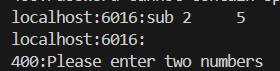
\includegraphics[width=0.5\linewidth]{figure/exception5.png}
    \caption{Extra space in the command}
\end{figure}

\section{Wireshark capture}

\begin{figure}[H]
    \centering
    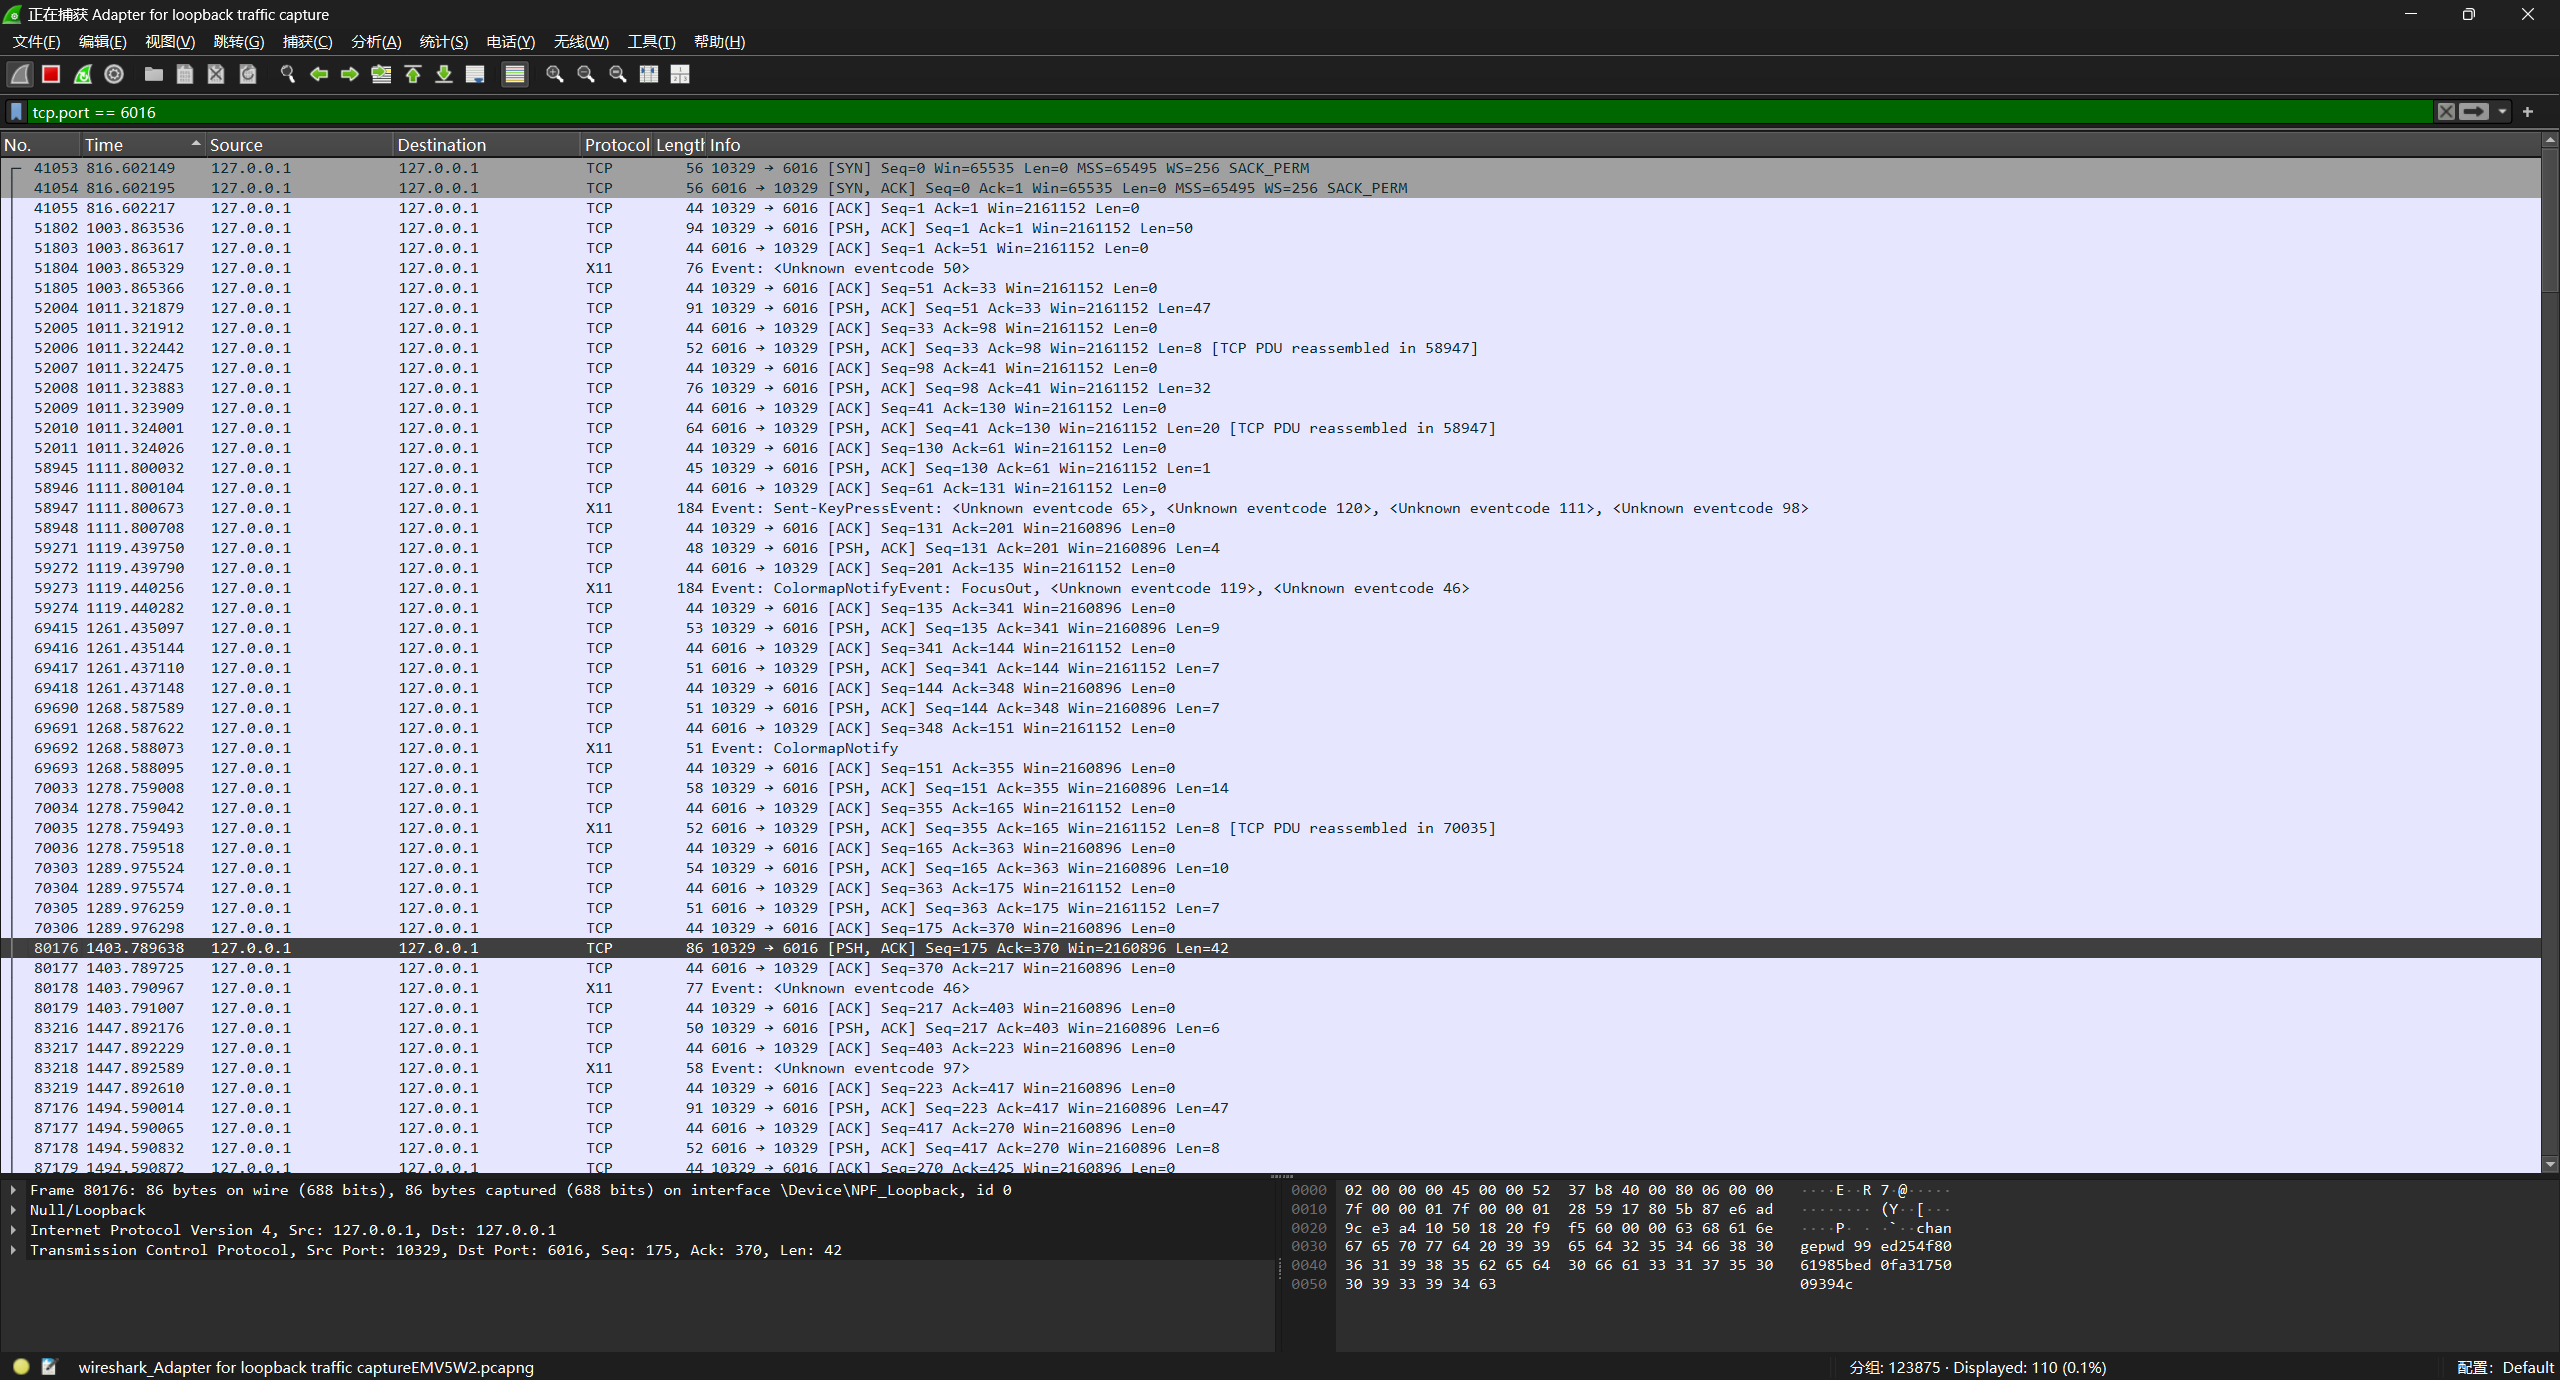
\includegraphics[width=\linewidth]{figure/wireshark.png}
    \caption{Part of the packet captured during the communication between the server and the client}
\end{figure}

\section{Code explanation}

Most code follows the instruction provided in the comments.
Only two parts requires further explanation.

\subsection{User Command Logging}

\begin{minted}{python}
def log_message(client_address, message, log_file="client_messages.txt"):
    with open(log_file, "a") as f:
        timestamp = time.strftime("%Y-%m-%d %H:%M:%S", time.localtime())
        f.write(f"[{timestamp}] {client_address}: {message}\n")

def main_loop(socket_conn, client_address, login_user):
    try:
        receive_data = socket_conn.recv(1024).decode('utf-8').strip()
        if not receive_data:
            return False, None
        else:
            log_message(client_address, receive_data)

    # process the command
\end{minted}

After receiving a message from the client, the server logs the message with the function \texttt{log\_message}.
All messages whether valid or invalid are logged, with the timestamp and the client address to distinguish them.
We append each log to the file \texttt{client\_messages.txt}.
This file manually does not need to be created manually, as the append mode will create it if it does not exist.

\subsection{Receiving challenge message}

\begin{minted}{python}
def generate_challenge():
    return os.urandom(8)

def server_response(server, password_hash):
    response = server.recv(1024)
    try:
        decoded_response = response.decode('utf-8')
        if decoded_response.startswith(('200:', '400:')):
            return response
        else:
            challenge_response = calculate_response(password_hash, response)
            server.send(challenge_response)
            return server.recv(1024)
    except UnicodeDecodeError:
        challenge_response = calculate_response(password_hash, response)
        server.send(challenge_response)
        return server.recv(1024)
\end{minted}

The \texttt{urandom} function generates 8 random bytes, which is the challenge message.
On the client side, we need to distinguish between the challenge message and a normal message.
We do this by checking the response in two steps, corresponding to the two major differences between the challenge message and a normal message.
Firstly, normal messages are encoded in UTF-8, while the challenge message is not.
Secondly, normal messages start with either \texttt{200:} or \texttt{400:}, while the challenge message does not.
Thus, we first try to decode the message with UTF-8, and then check if it starts with \texttt{200:} or \texttt{400:}.
Even in the rare case that the randomly generated challenge message is a valid UTF-8 string, it will very likely not start with \texttt{200:} or \texttt{400:}.

\end{document}